\documentclass[conference]{IEEEtran}

\usepackage{amsmath,amssymb}
\usepackage{graphicx}
\usepackage{booktabs}
\usepackage{cite}
\usepackage{url}
\usepackage[hidelinks]{hyperref}
\usepackage{multirow}

\begin{document}

\title{Hybrid-Sentinel: A Three-Tier Confidence-Gated AI Firewall for NDN Edge Deployment}

\author{
\IEEEauthorblockN{Raju Guguloth}
\IEEEauthorblockA{Indian Institute of Technology Madras\\
M.Tech Research --- TCL Collaboration\\
Email: \texttt{[your.email@iitm.ac.in]}}
}

\maketitle

\begin{abstract}
Signature-based intrusion detection systems such as Snort remain the backbone of network defense, yet their reliance on static, hand-maintained rule sets leaves them blind to novel attacks, prone to false alarms, and ill-suited to Named Data Networking (NDN) edge routers that forward discrete Interest/Data units rather than IP flows. This paper presents \textit{Hybrid-Sentinel}, a confidence-gated behavioural firewall that inspects 20-packet windows of 17 features and emits auditable \texttt{ALLOW}, \texttt{FLAG}, or \texttt{BLOCK} decisions. We evaluate the same methodological pattern on two complementary tracks. Track~A is a production three-tier cascade on Docker IP lab traffic: a 156\,KB Random Forest gate, a temperature-calibrated CNN-GRU (ONNX) over six attack classes, and a Mahalanobis one-class detector for zero-day novelty---achieving 100\% attack detection, 1.11\% benign false-positive rate, and 4.19\,ms mean CPU latency on 14{,}219 held-out sequences. Track~B is an NDN forwarder proof-of-concept that observes Pending Interest Table (PIT) and Content Store (CS) state to detect Interest Flooding and Cache Pollution, reaching 0.995 macro-F1 and 0.67\% benign FPR on 51{,}656 held-out windows. Together, the results show that a staged, learning-based design can outperform static signature engines on both IP-style behaviours and NDN-native attacks, while remaining explainable for edge operation.
\end{abstract}

\begin{IEEEkeywords}
Named Data Networking, intrusion detection, Snort, cascade classifier, Interest Flooding, Cache Pollution, ONNX, anomaly detection
\end{IEEEkeywords}

%----------------------------------------------------------------------
\section{Introduction}
\label{sec:intro}

Classical network intrusion detection is dominated by signature engines such as Snort and Suricata. These systems are fast at matching known patterns, but they fail when payloads are obfuscated, when attacks are novel, or when the protocol surface changes---problems that become acute at the NDN edge, where adversaries target forwarder state (Pending Interest Table exhaustion, Content Store pollution) rather than TCP/IP headers alone~\cite{ndn,afiha}. Deep learning detectors improve coverage, yet running a heavyweight model on every packet rarely fits a router latency budget.

Named Data Networking routes on content names and naturally inspects discrete Interest and Data packets at each hop~\cite{ndn}. This motivates a \emph{hybrid} firewall: a cheap gate on most traffic and a deeper model only when suspicion rises~\cite{tcl-wiki}. Hybrid-Sentinel implements that pattern and validates it on two tracks without conflating their evidence:
\begin{itemize}
\item \textbf{Track A (R18 production):} a three-tier cascade trained on controlled Docker TCP/IP PCAPs (brute force, HTTP flood, slow HTTP, port scan, DNS tunneling).
\item \textbf{Track B (NDN PoC):} the same behavioural-window idea applied to NDN-native features extracted from a simulated PIT+CS forwarder under Interest Flooding and Cache Pollution.
\end{itemize}

\paragraph{Contributions.}
(1)~A confidence-gated three-tier cascade with shared feature contract, ONNX deployment, and per-tier audit traces. (2)~Honest dual evaluation: IP lab cascade metrics plus transferable NDN-native detection of Interest Flooding and Cache Pollution. (3)~A reproducible build path from PCAP/simulation to FastAPI service suitable for edge research deployment.

%----------------------------------------------------------------------
\section{Related Work}
\label{sec:related}

Snort-style IDS relies on deterministic pattern matching and continuous rule maintenance; zero-day and protocol-native NDN attacks fall outside typical IP signature libraries~\cite{afiha}. Flow-based CNN/RNN IDS on public IP datasets (e.g., CIC-IDS) demonstrates deep models on packet sequences~\cite{cicids} but does not address NDN forwarder state. Prior NDN security work studies Interest Flooding against the PIT and pollution against the CS~\cite{afiha,compagno}. Our contribution is a \emph{confidence-gated cascade} for production IP behaviours, plus a PoC showing that windowed behavioural features transfer to NDN state observations---without claiming the IP models were trained on NDN packets.

%----------------------------------------------------------------------
\section{System Architecture}
\label{sec:system}

Fig.~\ref{fig:unified} summarises the dual-track design. Both tracks share a detection method---17 features organised as 20-packet windows feeding a confidence-aware classifier---but differ in feature semantics and model stack.

\begin{figure*}[!t]
\centering
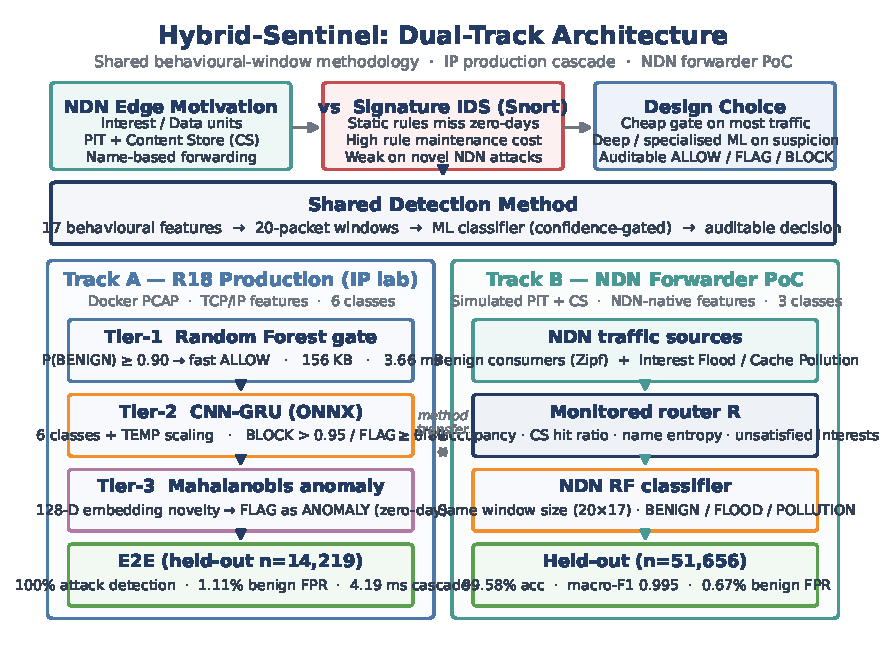
\includegraphics[width=\textwidth]{figures/fig_unified_system_architecture.pdf}
\caption{Hybrid-Sentinel dual-track architecture. Track~A is the R18 production cascade on IP lab PCAPs. Track~B transfers the same windowed methodology to NDN PIT/CS observations (simulation).}
\label{fig:unified}
\end{figure*}

\subsection{Track A: R18 runtime cascade}
Each decision uses a scaled window $\mathbf{X} \in \mathbb{R}^{20 \times 17}$. Tier-1 summarises the window (mean, standard deviation, last packet) and estimates $P(\text{BENIGN})$; above $\tau_1{=}0.90$ the window is \texttt{ALLOW}ed without deep inference. Otherwise Tier-2 (CNN-GRU, temperature-scaled) assigns one of six labels; confidence above $\tau_b{=}0.95$ yields \texttt{BLOCK}, and $[\tau_f,\tau_b)$ with $\tau_f{=}0.80$ yields \texttt{FLAG}. Tier-3 scores Mahalanobis distance on a 128-D embedding and may \texttt{FLAG} residual novelty as \texttt{ANOMALY}. Fig.~\ref{fig:arch} details the decision flow; Fig.~\ref{fig:orch} shows build orchestration from capture through ONNX export to the FastAPI service.

\begin{figure}[!t]
\centering
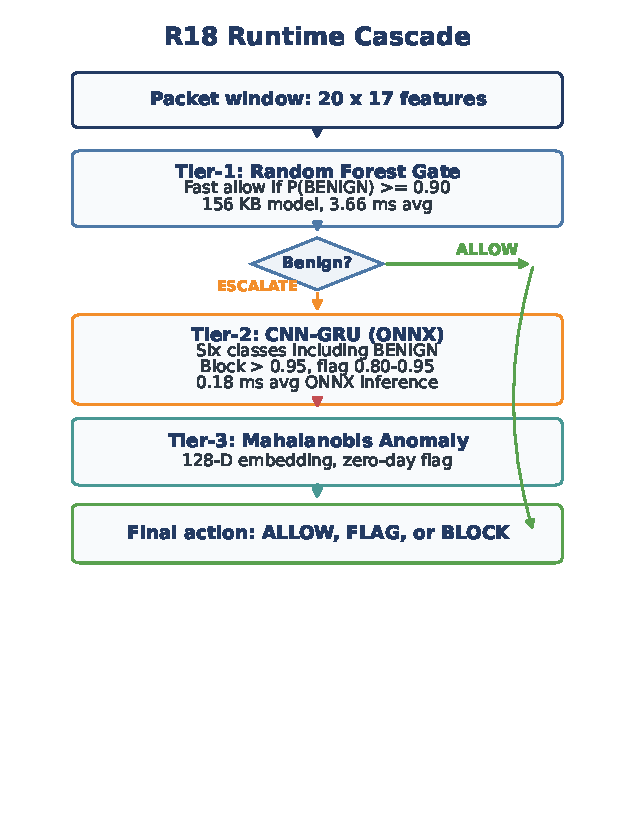
\includegraphics[width=\columnwidth]{figures/architecture_flow.pdf}
\caption{Track~A runtime three-tier decision flow. Fast-path \texttt{ALLOW} skips deep inference when Tier-1 benign confidence is high.}
\label{fig:arch}
\end{figure}

\begin{figure}[!t]
\centering
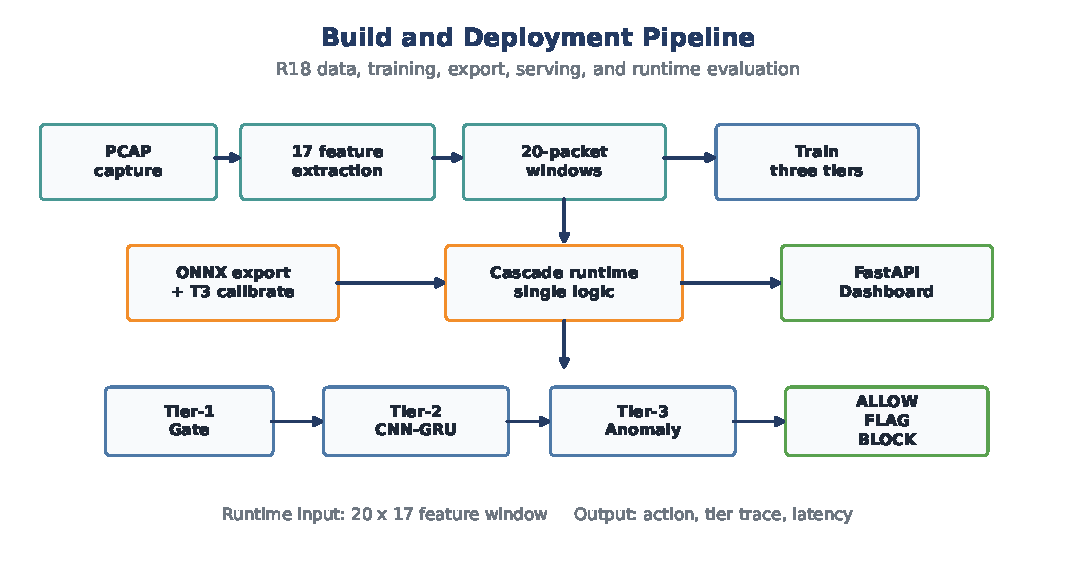
\includegraphics[width=\columnwidth]{figures/orchestration_pipeline.pdf}
\caption{Track~A build orchestration: capture, feature extraction, training, ONNX export, unified cascade, API.}
\label{fig:orch}
\end{figure}

\subsection{Track B: NDN forwarder PoC}
Fig.~\ref{fig:ndn_topo} shows the simulated topology. Benign consumers issue Zipf-popular Interests; attackers inject unsatisfiable names (Interest Flooding $\rightarrow$ PIT exhaustion) or cold catalog names (Cache Pollution $\rightarrow$ CS hit-ratio collapse). The observation point is router~$R$ (PIT+CS). Seventeen NDN-native features (e.g., PIT size growth, CS hit ratio, name entropy, unsatisfied Interest ratio) form 20-packet windows classified as \texttt{BENIGN}, \texttt{INTEREST\_FLOODING}, or \texttt{CACHE\_POLLUTION}.

\begin{figure}[!t]
\centering
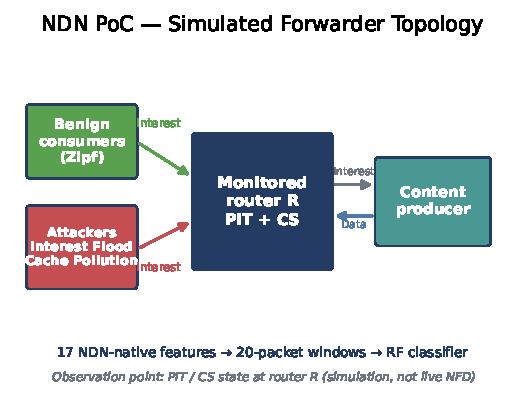
\includegraphics[width=\columnwidth]{figures/fig_ndn_architecture.pdf}
\caption{Track~B simulated NDN topology. Interest/Data exchange is observed at router~$R$ (PIT + Content Store); this is a discrete-event simulation, not a live NFD testbed.}
\label{fig:ndn_topo}
\end{figure}

%----------------------------------------------------------------------
\section{Methodology}
\label{sec:method}

\subsection{Track A features and training}
Seventeen packet-level IP features (length, protocol flags, payload entropy, flow aggregates) are extracted with Scapy. Sliding windows of size 20 (stride 10) form sequences. Sequences are grouped by pseudo-flow blocks; train/validation/test splits are 70/15/15 with zero group overlap. The scaler is fit on training data only. Tier-2 uses focal loss with elevated benign weight and temperature calibration on validation. Tier-3 is fit on benign training embeddings and must be re-exported when Tier-2 weights change. Tier-2 inference uses ONNX Runtime on CPU; cascade logic lives in a single module shared by evaluation and the API.

\subsection{Track B NDN features}
NDN features deliberately parallel the production 17-dimensional contract but read forwarder state: Interest/Data indicators, name depth and entropy, PIT occupancy and growth, CS size and hit signals, interarrival and windowed rates. Features are causal (past observations only), so the extractor is conceptually deployable on a live forwarder. A Random Forest classifier is trained with a stratified 75/25 train/test split on simulated windows.

%----------------------------------------------------------------------
\section{Experimental Setup}
\label{sec:setup}

\paragraph{Track A.}
Traffic was generated in an isolated Docker bridge network with producer containers (HTTP, SSH, DNS) and scripted attackers. The held-out test set contains 14{,}219 sequences (814 benign, 13{,}405 attack) never used for training or model selection. Latency is measured over 2{,}000 CPU inferences (single-threaded Tier-1).

\paragraph{Track B.}
A discrete-event NDN simulator emits 206{,}624 windows (43{,}299 BENIGN, 63{,}308 INTEREST\_FLOODING, 100{,}017 CACHE\_POLLUTION). Held-out evaluation uses 51{,}656 windows. Absolute numbers reflect simulator assumptions (Poisson arrivals, Zipf popularity, LRU CS, fixed PIT lifetime) and complement---not replace---Track~A.

%----------------------------------------------------------------------
\section{Results}
\label{sec:results}

\subsection{Track A: per-tier and end-to-end}
Table~\ref{tab:tier} lists per-component metrics. Tier-1 separates benign fast-path from attack escalation with zero benign false escalations on the test set. Tier-2 macro-F1 is 0.985; \texttt{BRUTE\_FORCE} has the lowest recall (0.914) due to early-packet overlap with slow HTTP. The full cascade detects all 13{,}405 attacks (100\%) and falsely flags 9 of 814 benign windows (1.11\% FPR); none are auto-blocked without review.

\begin{table}[!t]
\caption{Track~A (R18) per-tier metrics on held-out test ($n{=}14{,}219$). Tier-2 uses macro averaging.}
\label{tab:tier}
\centering
\small
\begin{tabular}{lccccc}
\toprule
\textbf{Component} & \textbf{Acc.} & \textbf{Prec.} & \textbf{Rec.} & \textbf{F1} & \textbf{Latency} \\
\midrule
Tier-1 gate       & 1.000 & 1.000 & 1.000 & 1.000 & 3.66\,ms \\
Tier-2 CNN-GRU    & 0.981 & 0.986 & 0.985 & 0.985 & 0.18\,ms \\
Tier-3 anomaly    & 0.995 & 0.992 & 1.000 & 0.996 & 0.21\,ms \\
Full cascade      & 0.999 & 0.999 & 1.000 & 1.000 & 4.19\,ms \\
\bottomrule
\end{tabular}
\vspace{2pt}
\parbox{\linewidth}{\footnotesize Throughput: Tier-1 272\,seq/s; Tier-2 ONNX 5{,}570\,seq/s; full cascade 238\,seq/s. Baseline gradient-boosting latency $\approx$13\,ms.}
\end{table}

Fig.~\ref{fig:metrics}--\ref{fig:heatmap} summarise Track~A discrimination; Fig.~\ref{fig:e2e}--\ref{fig:funnel} show security outcomes and cascade load; Fig.~\ref{fig:lat} reports latency/throughput.

\begin{figure}[!t]
\centering
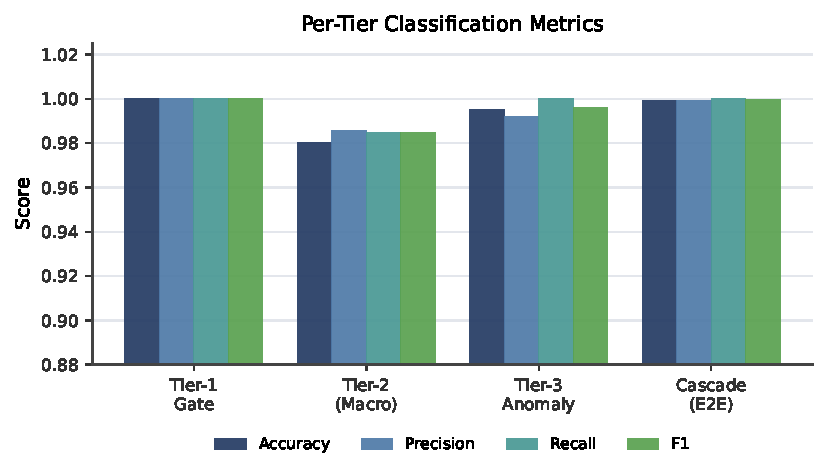
\includegraphics[width=\columnwidth]{figures/tier_metrics_bars.pdf}
\caption{Track~A accuracy, precision, recall, and F1 across tiers and end-to-end cascade.}
\label{fig:metrics}
\end{figure}

\begin{figure}[!t]
\centering
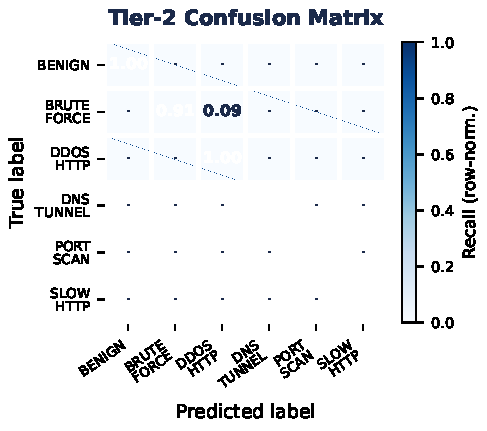
\includegraphics[width=\columnwidth]{figures/confusion_matrix.pdf}
\caption{Track~A Tier-2 normalised confusion matrix (single-column layout).}
\label{fig:cm}
\end{figure}

\begin{figure}[!t]
\centering
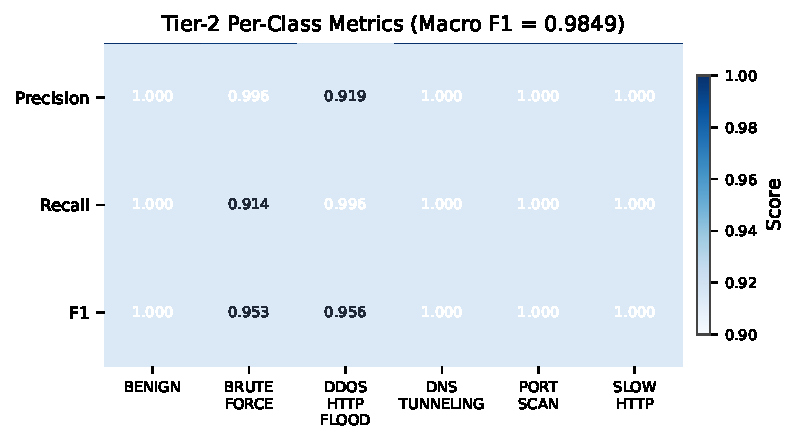
\includegraphics[width=\columnwidth]{figures/per_class_heatmap.pdf}
\caption{Track~A Tier-2 per-class precision, recall, and F1.}
\label{fig:heatmap}
\end{figure}

\begin{figure}[!t]
\centering
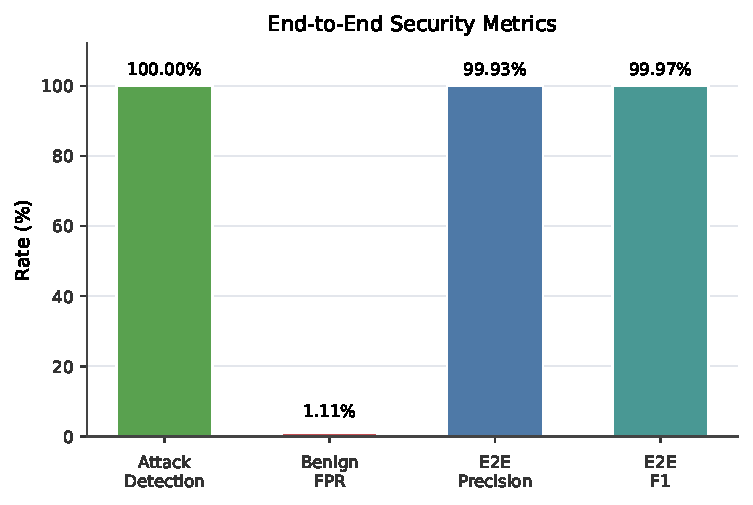
\includegraphics[width=\columnwidth]{figures/e2e_security.pdf}
\caption{Track~A end-to-end attack detection, benign FPR, precision, and F1.}
\label{fig:e2e}
\end{figure}

\begin{figure}[!t]
\centering
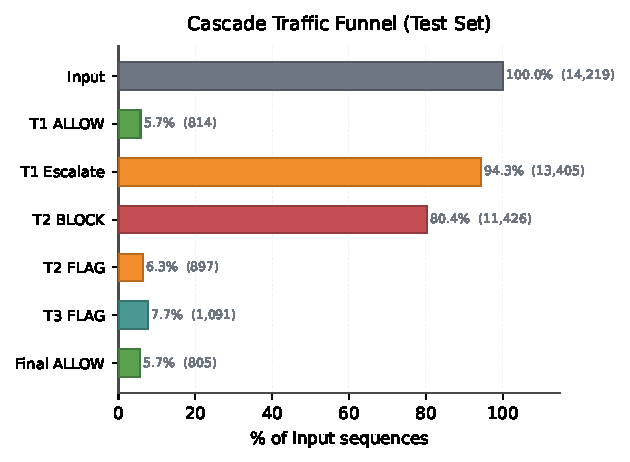
\includegraphics[width=\columnwidth]{figures/cascade_funnel.pdf}
\caption{Track~A cascade funnel: percentage of sequences at each stage.}
\label{fig:funnel}
\end{figure}

\begin{figure}[!t]
\centering
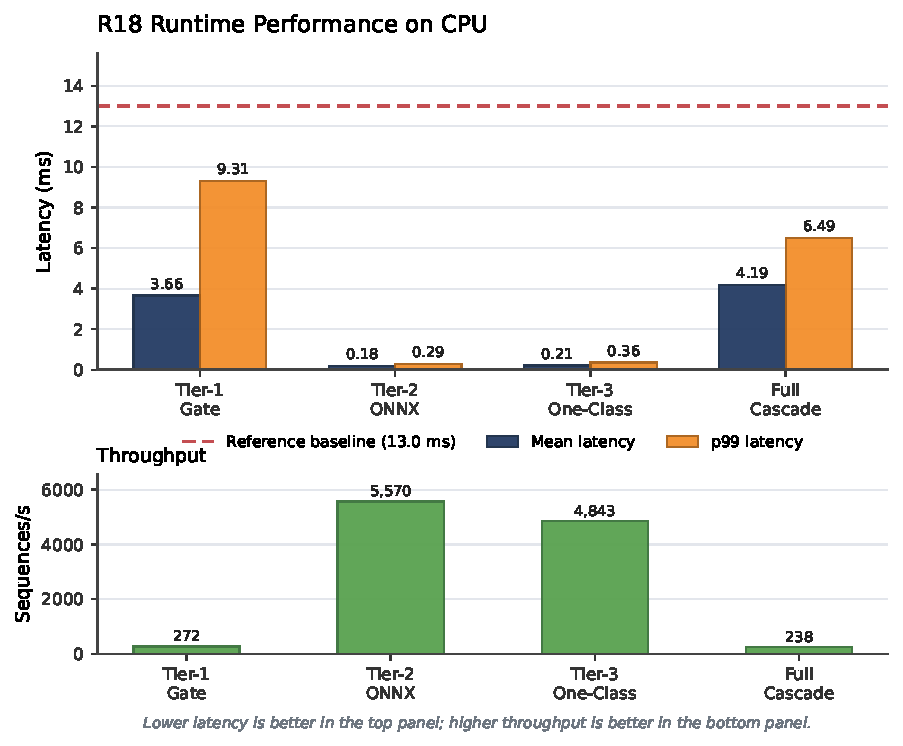
\includegraphics[width=\columnwidth]{figures/latency_throughput.pdf}
\caption{Track~A inference latency and throughput (CPU, $n{=}2000$). Dashed line: 13\,ms gradient-boosting reference.}
\label{fig:lat}
\end{figure}

\subsection{Track B: NDN PoC}
Table~\ref{tab:ndn} and Fig.~\ref{fig:ndn_cm}--\ref{fig:ndn_summary} report held-out NDN results. Interest Flooding is perfectly separable (PIT-exhaustion signature). Residual errors are a small BENIGN~$\leftrightarrow$~CACHE\_POLLUTION overlap during low-density attack warmup---expected under Zipf/LRU dynamics.

\begin{table}[!t]
\caption{Track~B NDN PoC held-out metrics ($n{=}51{,}656$).}
\label{tab:ndn}
\centering
\small
\begin{tabular}{lcccc}
\toprule
\textbf{Class / Aggregate} & \textbf{Prec.} & \textbf{Rec.} & \textbf{F1} & \textbf{Acc.} \\
\midrule
BENIGN & 0.987 & 0.993 & 0.990 & 0.993 \\
CACHE\_POLLUTION & 0.997 & 0.994 & 0.996 & 0.994 \\
INTEREST\_FLOODING & 1.000 & 1.000 & 1.000 & 1.000 \\
\midrule
Overall & --- & --- & 0.995 & 0.996 \\
\bottomrule
\end{tabular}
\vspace{2pt}
\parbox{\linewidth}{\footnotesize Attack detection 99.65\%; benign FPR 0.67\%; ROC-AUC (attack vs.\ benign) 0.9997.}
\end{table}

\begin{figure}[!t]
\centering
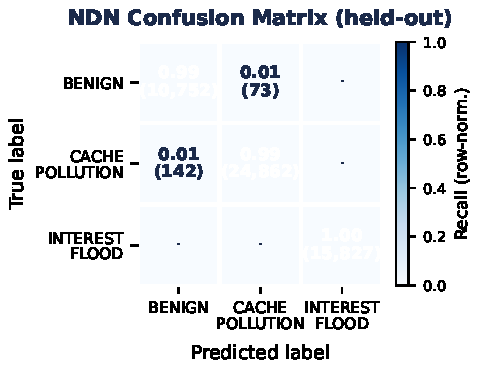
\includegraphics[width=\columnwidth]{figures/fig_ndn_confusion_matrix.pdf}
\caption{Track~B normalised confusion matrix (counts in parentheses; single-column).}
\label{fig:ndn_cm}
\end{figure}

\begin{figure}[!t]
\centering
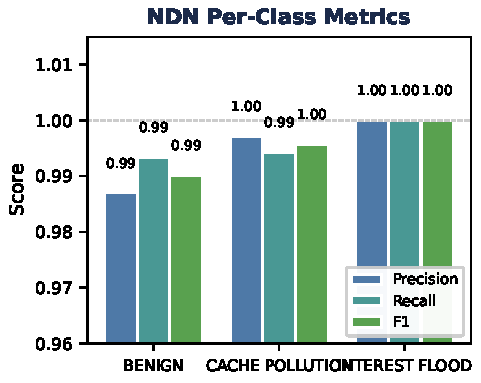
\includegraphics[width=\columnwidth]{figures/fig_ndn_per_class_metrics.pdf}
\caption{Track~B per-class precision, recall, and F1.}
\label{fig:ndn_metrics}
\end{figure}

\begin{figure}[!t]
\centering
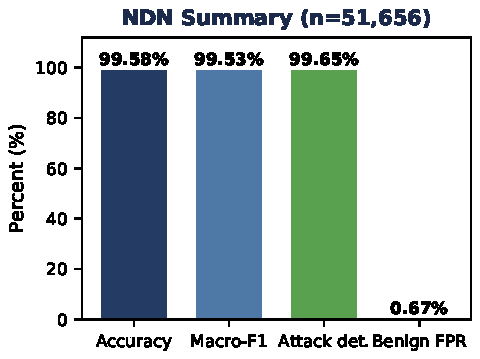
\includegraphics[width=\columnwidth]{figures/fig_ndn_summary_metrics.pdf}
\caption{Track~B summary metrics on held-out windows.}
\label{fig:ndn_summary}
\end{figure}

\begin{figure}[!t]
\centering
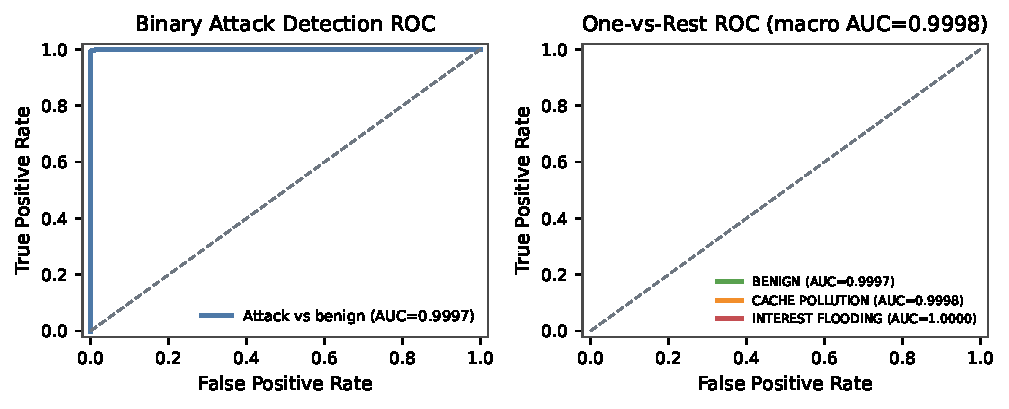
\includegraphics[width=\linewidth]{figures/fig_ndn_roc_curves.pdf}
\caption{Track~B ROC: binary attack detection (left) and one-vs-rest (right).}
\label{fig:ndn_roc}
\end{figure}

%----------------------------------------------------------------------
\section{Discussion}
\label{sec:discuss}

Relative to Snort-like static rules, Hybrid-Sentinel learns behavioural windows and can FLAG novelty without waiting for a new signature. Track~A shows that cascading a cheap gate with calibrated deep classification and embedding anomaly detection meets edge latency budgets on CPU. Track~B shows the \emph{methodology} transfers when features are redefined for PIT/CS state.

\paragraph{Limitations.}
Track~B is a simulation, not a live NFD/ndnSIM capture. Track~A remains IP-overlay lab traffic; enterprise TLS and live NDN malware-in-Data remain future work. The paper deliberately separates the two tracks to avoid overclaiming that production cascade weights were trained on NDN packets.

%----------------------------------------------------------------------
\section{Conclusion}
\label{sec:concl}

Hybrid-Sentinel delivers a reproducible, confidence-gated AI firewall: 100\% attack detection with 1.11\% benign FPR and 4.19\,ms cascade latency on IP lab traffic, plus an NDN PoC that detects Interest Flooding and Cache Pollution at 0.995 macro-F1. By pairing a Snort-motivated critique with dual-track evidence, we show that hybrid behavioural detection is a practical path toward NDN edge defense.

\section*{Acknowledgment}
The author thanks the TCL--IITM research collaboration for infrastructure and technical guidance.

\begin{thebibliography}{00}
\bibitem{tcl-wiki}
T.~Sood \textit{et al.},
``Next-Generation Firewall Architectures: Rule-Based vs.\ AI Transformers,''
TCL--IITM GitLab Wiki, 2026.

\bibitem{ndn}
L.~Zhang \textit{et al.},
``Named Data Networking,''
\emph{ACM SIGCOMM CCR}, vol.~44, no.~3, pp.~66--73, 2014.

\bibitem{afiha}
A.~Compagno \textit{et al.},
``Poseidon: Mitigating Interest Flooding DDoS Attacks in Named Data Networking,''
\emph{Proc.\ IEEE LCN}, 2013.

\bibitem{cicids}
I.~Sharafaldin \textit{et al.},
``Toward Generating a New Intrusion Detection Dataset and Intrusion Traffic Characterization,''
\emph{Proc.\ ICISSp}, 2018.
\end{thebibliography}

\end{document}
